\chapter{Документация к ATmega8}
\label{appendmk}
% \includepdf[angle=45,pages={3}]{atmega_dh.pdf}
% \includepdf[pages={1-2}]{atmega_dh.pdf}
% \includepdf[pages={1-2},offset=75 -75]{atmega_dh.pdf}
\begin{figure}[ht]
	\centering
	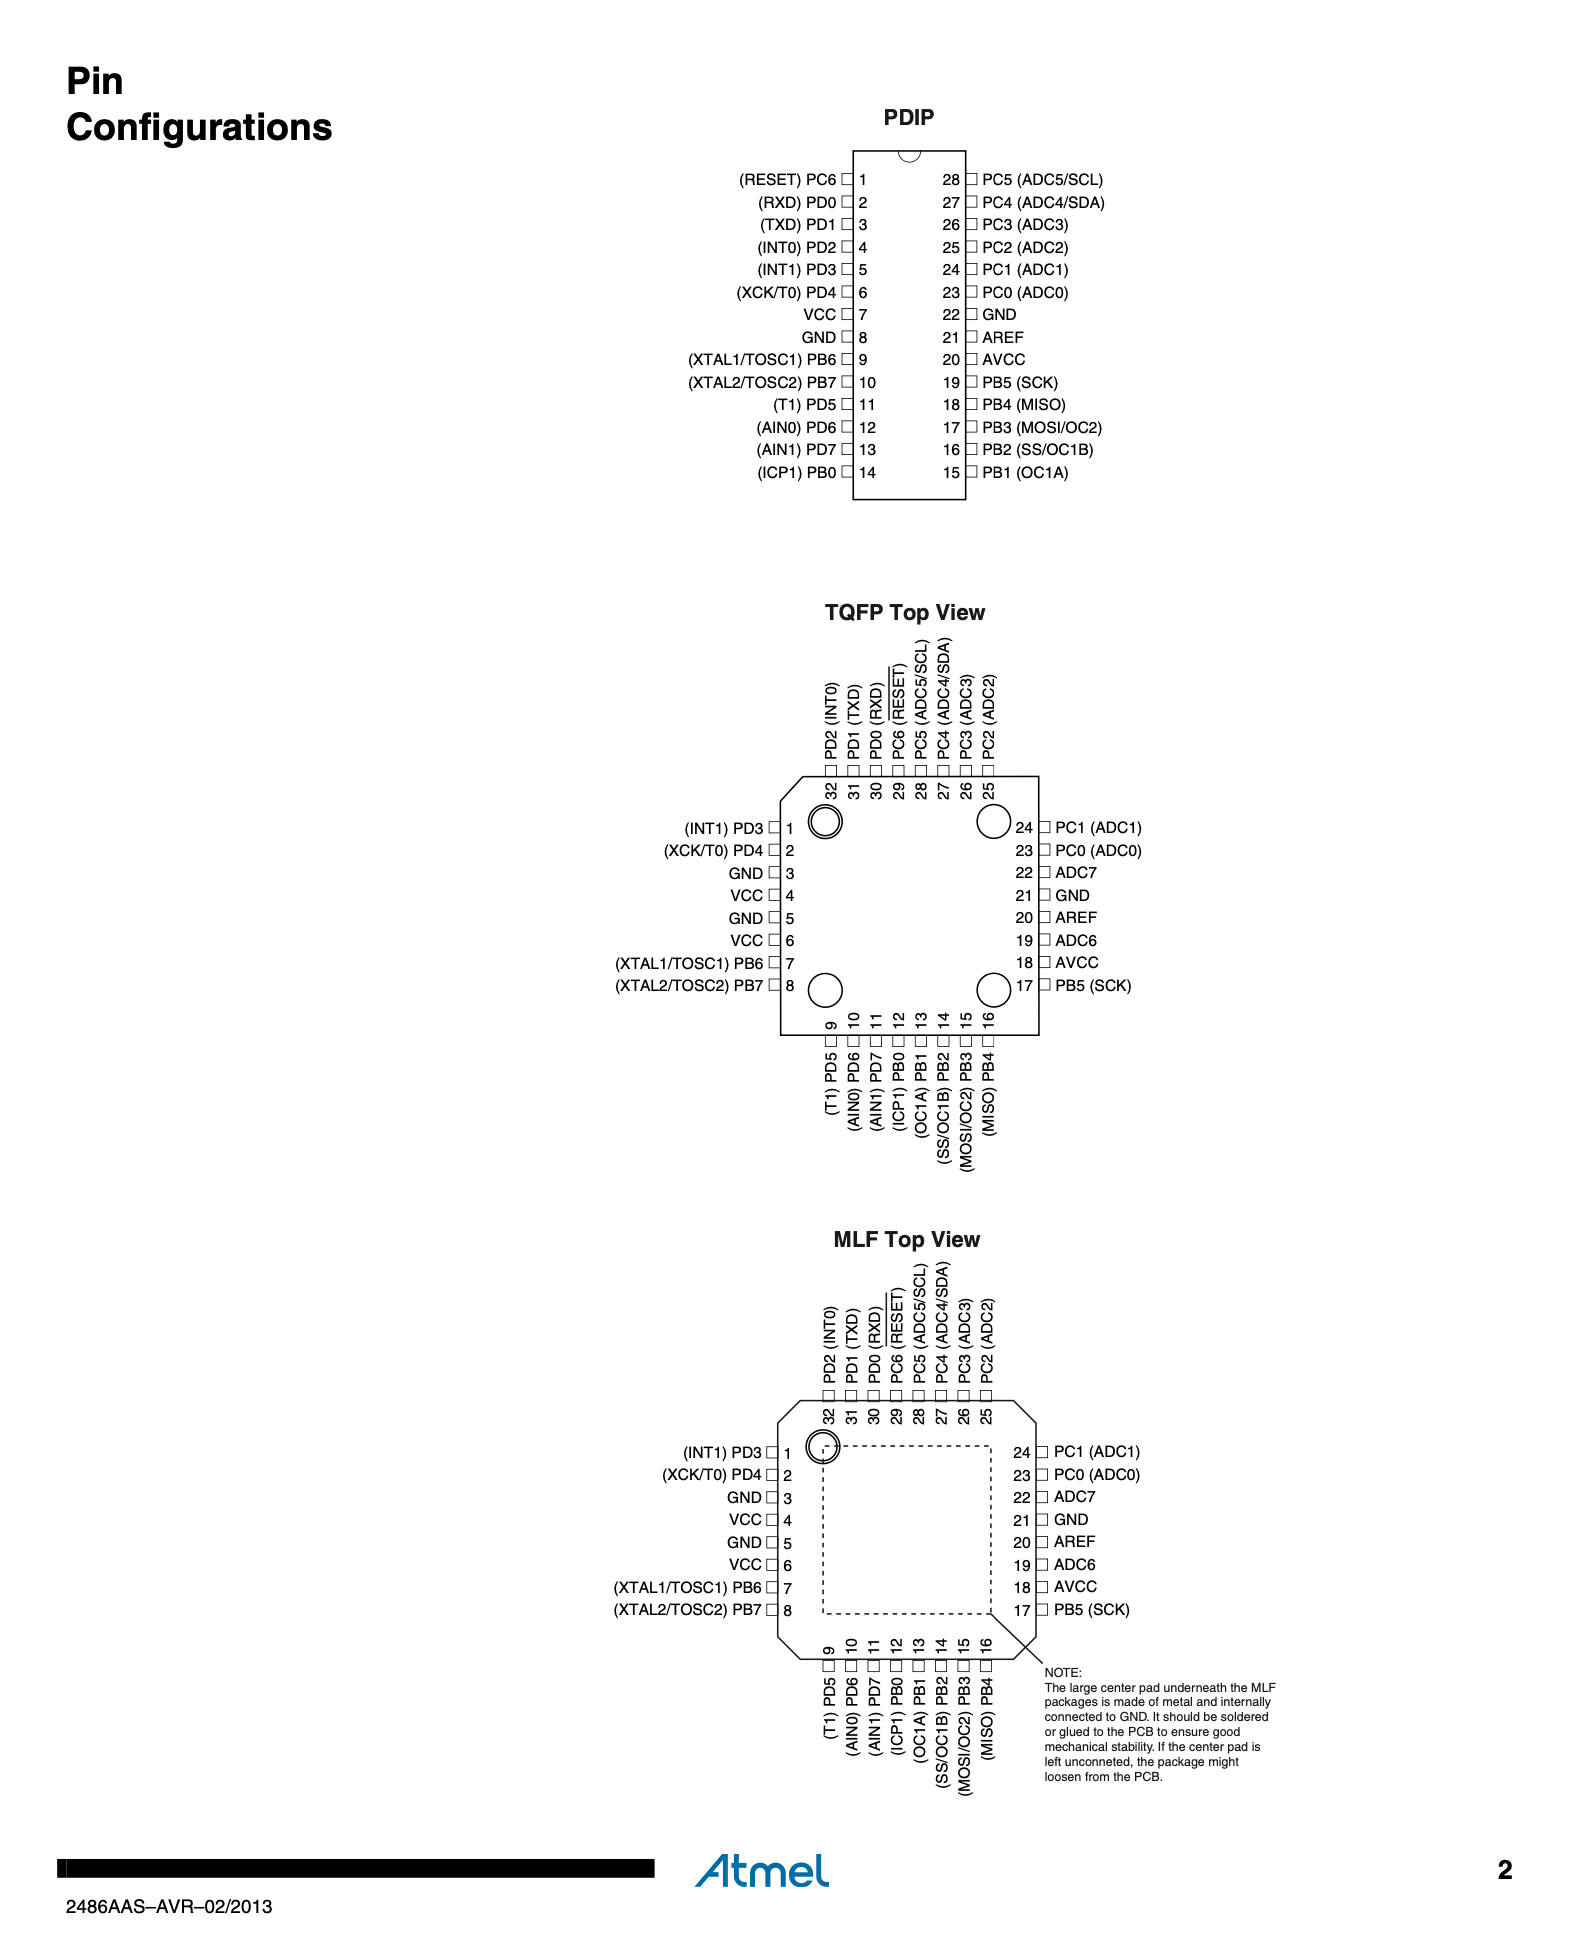
\includegraphics[width=0.9\textwidth]{./images/atmega_dh1.png}
	% \caption{Функциональная схема устройства: ИП -- источник питания; БП -- блок питания; Д -- датчик; ОУ -- операционный усилитель; АЦП -- аналого-цифровой преобразователь; МК -- микроконтроллер; ЭПУ -- электрическое преобразовательное устройство; ГВЧ -- высокочастотный генератор; Ф -- RC-фильтр; МВ -- мостовой выпрямитель;}
	\label{fig:atmega}
\end{figure}
% \begin{figure}[ht]
% 	\centering
% 	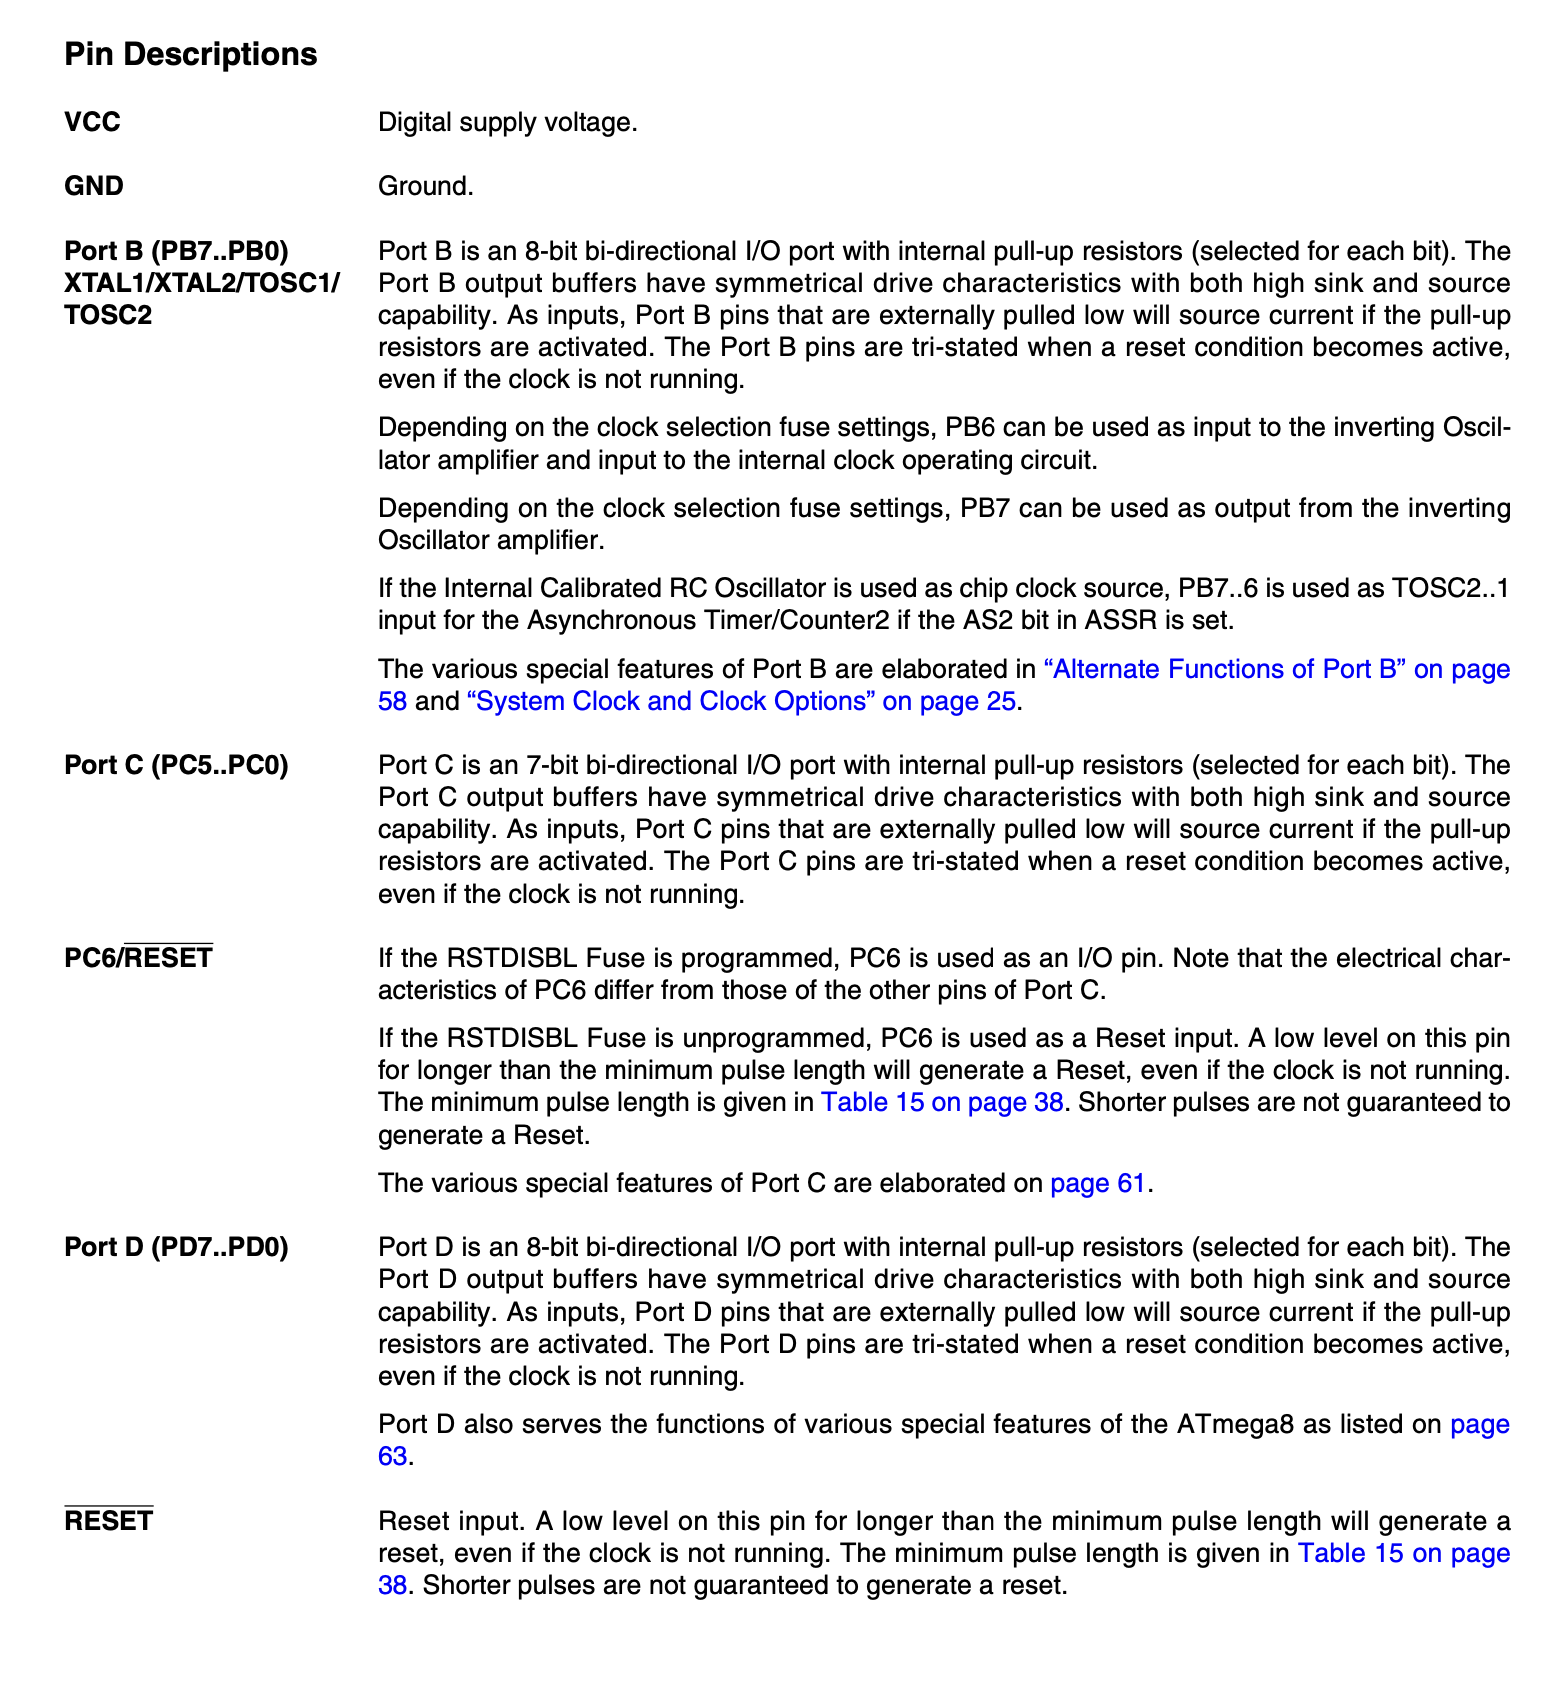
\includegraphics[width=\textwidth]{./images/atmega_dh2.png}
% 	% \caption{Функциональная схема устройства: ИП -- источник питания; БП -- блок питания; Д -- датчик; ОУ -- операционный усилитель; АЦП -- аналого-цифровой преобразователь; МК -- микроконтроллер; ЭПУ -- электрическое преобразовательное устройство; ГВЧ -- высокочастотный генератор; Ф -- RC-фильтр; МВ -- мостовой выпрямитель;}
% 	\label{fig:atmega2}
% \end{figure}


% \chapter{Документация к операционному усилителю}
% \label{appendmult}
% \begin{figure}[ht]
% 	\centering
% 	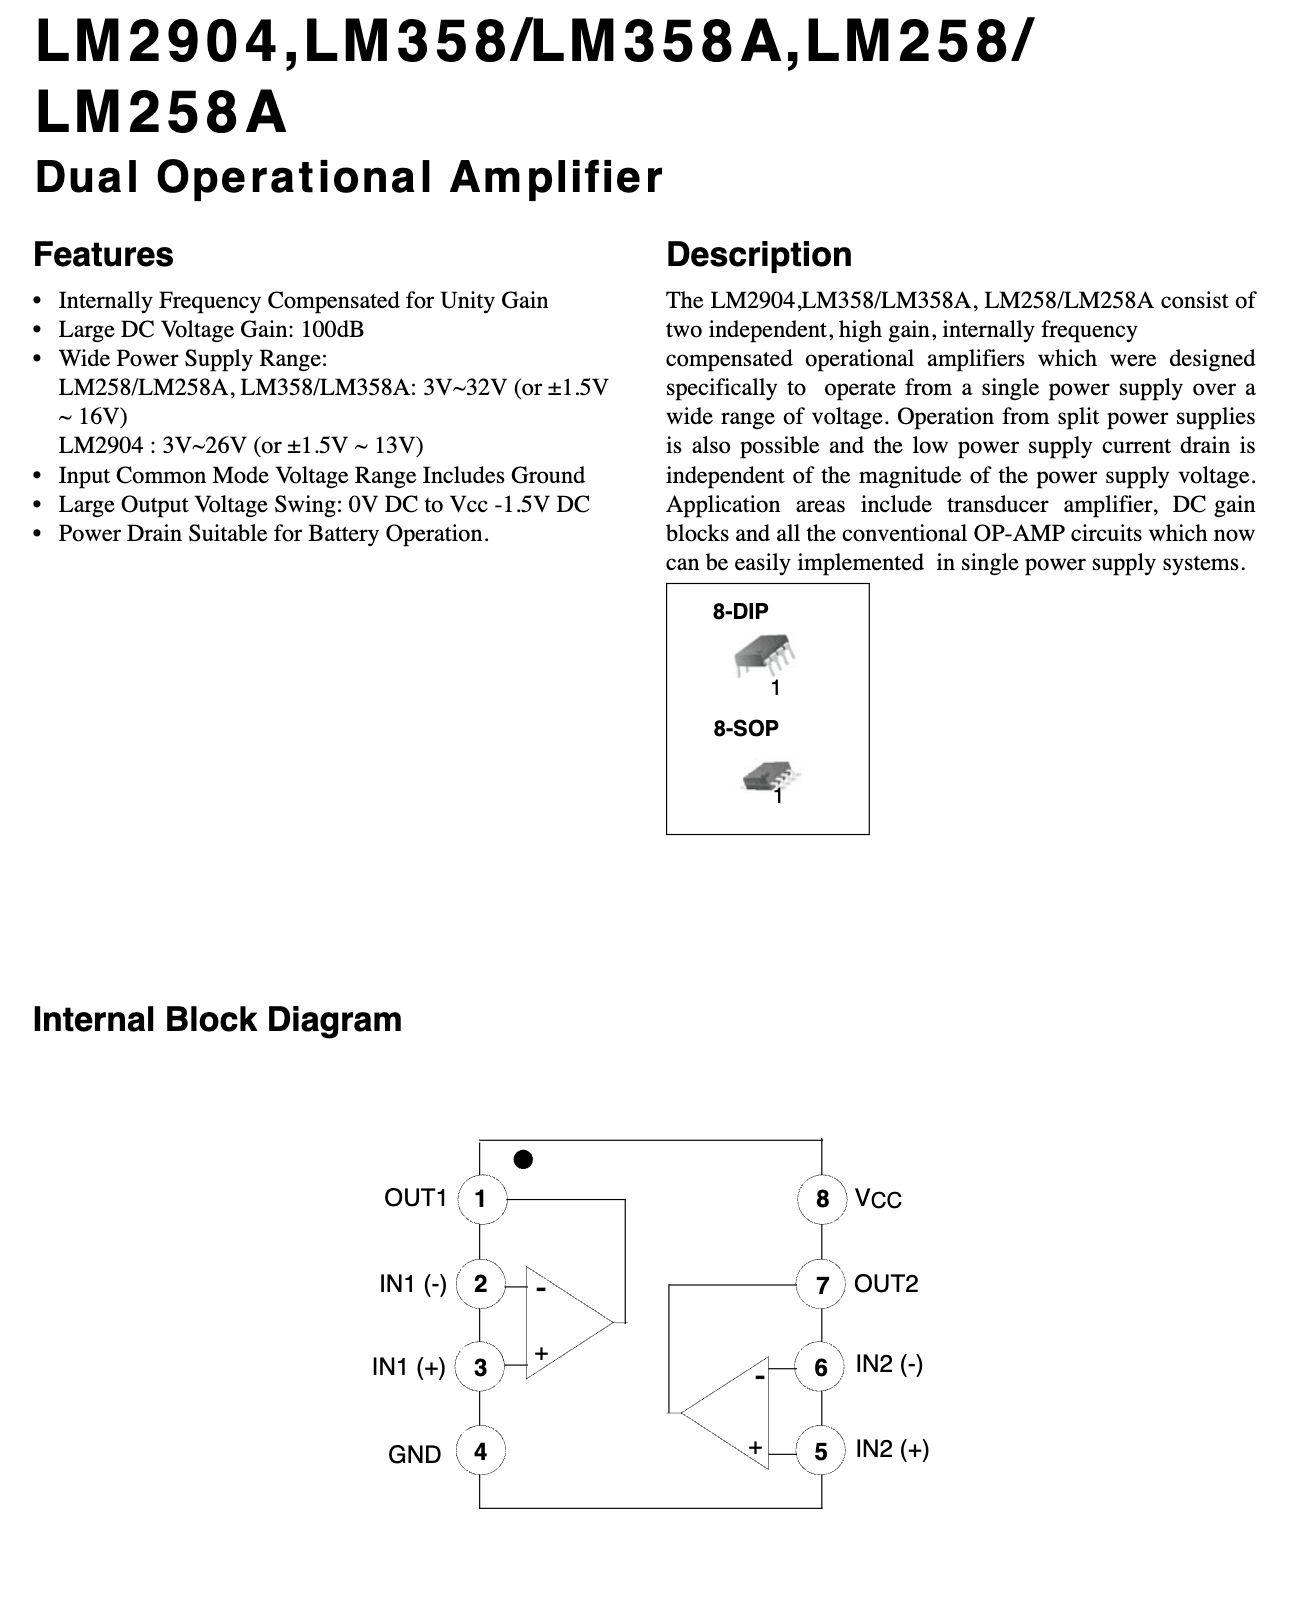
\includegraphics[width=0.8\textwidth]{./images/ou.png}
% 	% \caption{Функциональная схема устройства: ИП -- источник питания; БП -- блок питания; Д -- датчик; ОУ -- операционный усилитель; АЦП -- аналого-цифровой преобразователь; МК -- микроконтроллер; ЭПУ -- электрическое преобразовательное устройство; ГВЧ -- высокочастотный генератор; Ф -- RC-фильтр; МВ -- мостовой выпрямитель;}
% 	\label{fig:ou}
% \end{figure}


% \chapter{Документация к ГВЧ}
% \label{appendgenerator}
% \begin{figure}[ht]
% 	\centering
% 	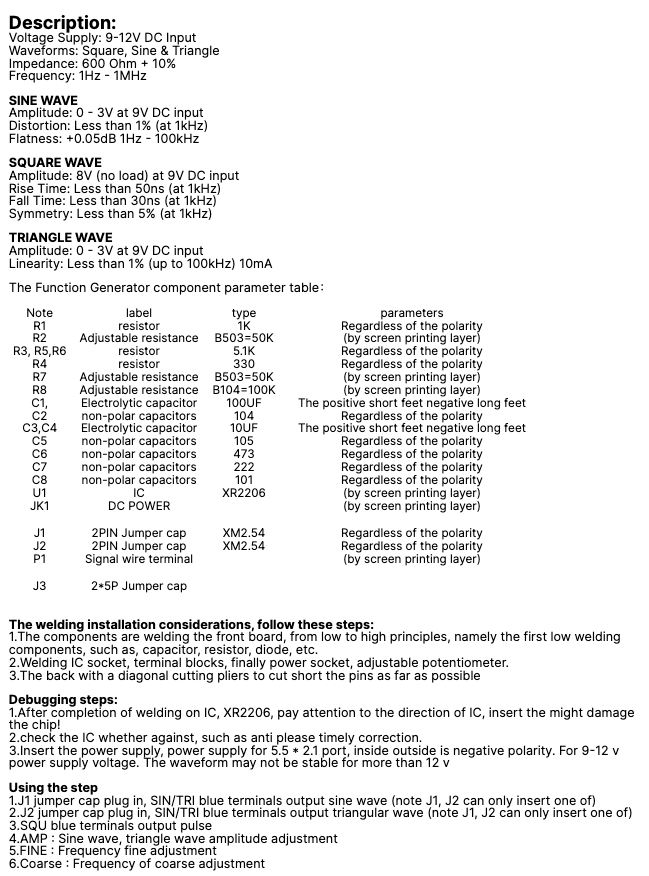
\includegraphics[width=0.8\textwidth]{./images/generator.png}
% 	% \caption{Функциональная схема устройства: ИП -- источник питания; БП -- блок питания; Д -- датчик; ОУ -- операционный усилитель; АЦП -- аналого-цифровой преобразователь; МК -- микроконтроллер; ЭПУ -- электрическое преобразовательное устройство; ГВЧ -- высокочастотный генератор; Ф -- RC-фильтр; МВ -- мостовой выпрямитель;}
% 	\label{fig:generator}
% \end{figure}


% \chapter{Документация к блоку питания}
% \label{appendbp}
% \begin{figure}[ht]
% 	\centering
% 	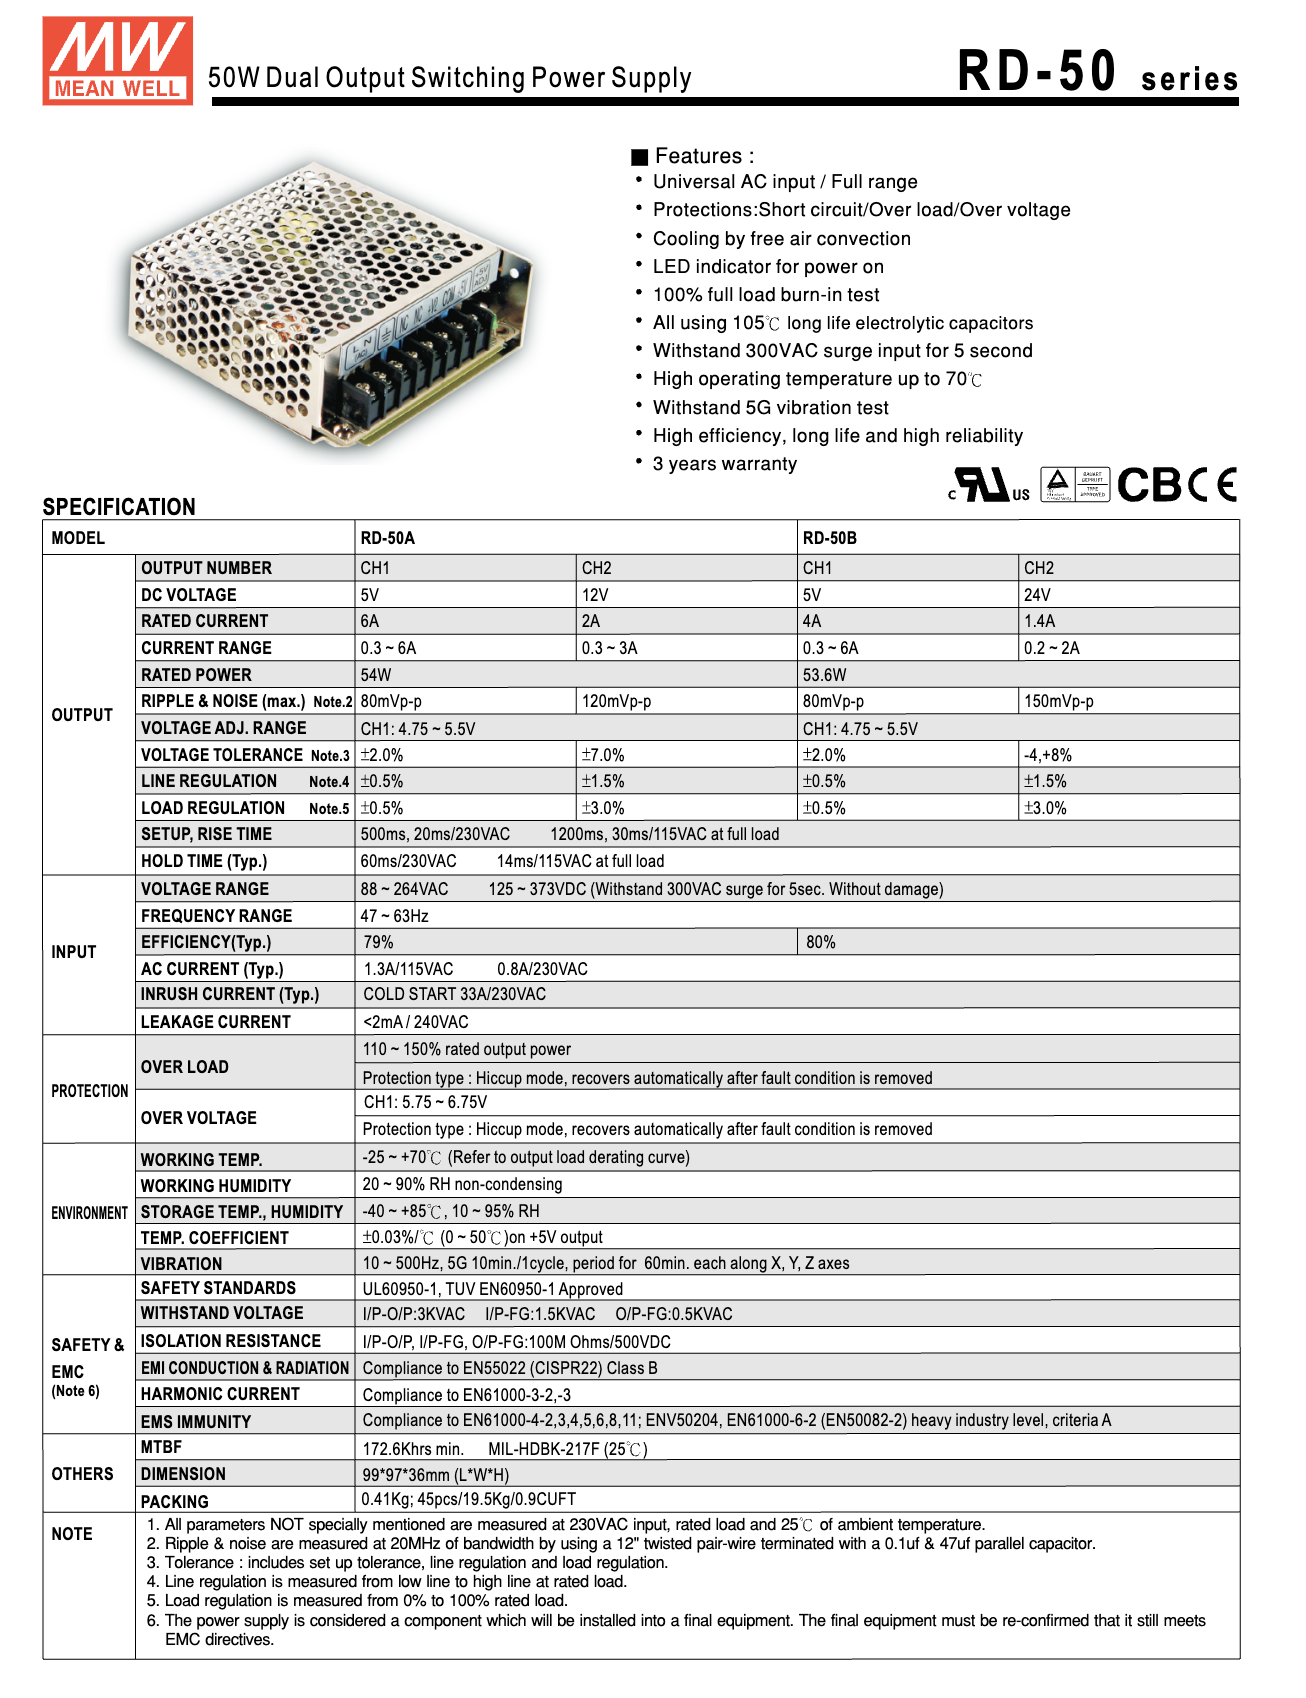
\includegraphics[width=0.9\textwidth]{./images/bp.png}
% 	% \caption{Функциональная схема устройства: ИП -- источник питания; БП -- блок питания; Д -- датчик; ОУ -- операционный усилитель; АЦП -- аналого-цифровой преобразователь; МК -- микроконтроллер; ЭПУ -- электрическое преобразовательное устройство; ГВЧ -- высокочастотный генератор; Ф -- RC-фильтр; МВ -- мостовой выпрямитель;}
% 	\label{fig:bp1}
% \end{figure}

% \chapter{Перечень элементов}
% \label{appendlist}
% \begin{figure}[ht]
% 	\centering
% 	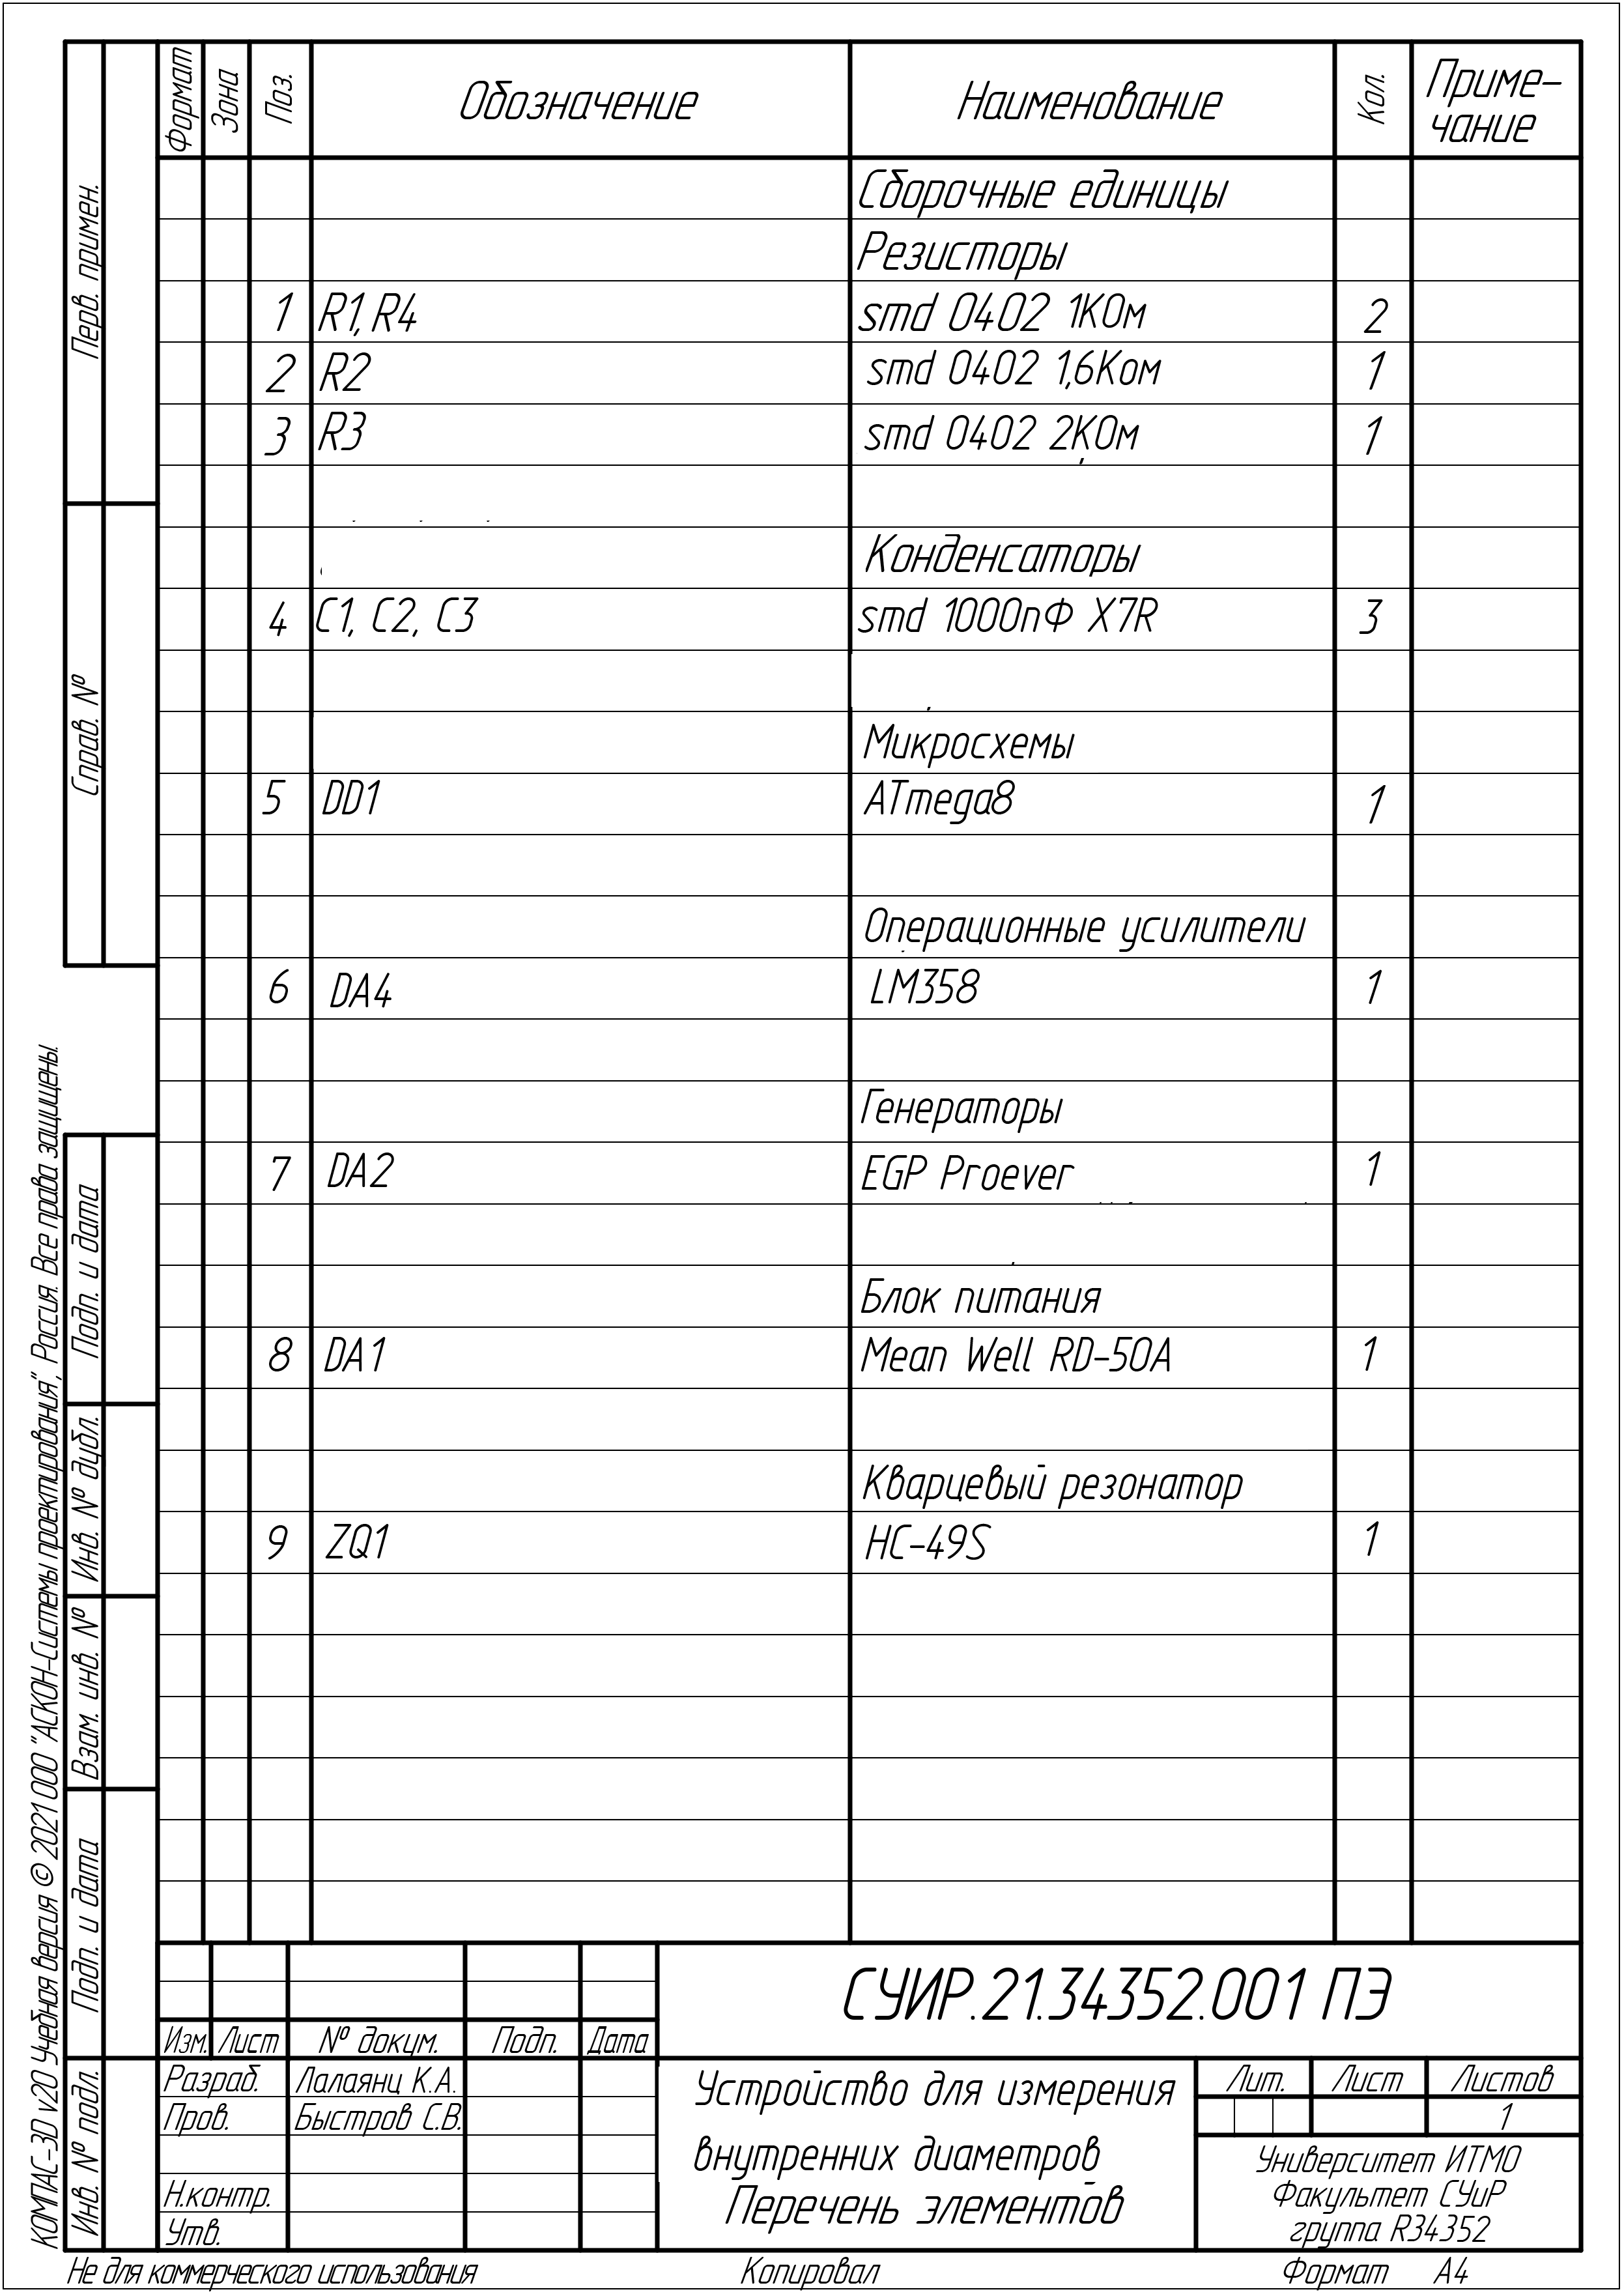
\includegraphics[width=0.9\textwidth]{./images/Список.png}
% 	% \caption{Схема подключения к МК: ИП -- источник питания; Д -- датчик; Z1 -- кварцевый ГВЧ; VD1...4 диоды; C1...C3 -- конденсаторы; R1...R4 -- резисторы; ОУ -- операционный усилитель;}
% 	\label{fig:list}
% \end{figure}